
\section{Real-Time Scheduling}
\begin{description}
    \item[Job/processes/threads]: A task to be executed which compete for
        limited resource, the CPU
    \item[Scheduling:] Given N jobs, in which order should the CPU execute
        them
\end{description}

\paragraph{Scheduling goals}:

\begin{tabular}{lm{0.45\linewidth}m{0.45\linewidth}}
    & In general purposes OS( Linux,Windows, \ldots) &
    Real-time OS \\
    &
    \begin{description}
        \item[Fairness] All jobs should be finally executed (no starvation)
        \item[Optimize response time] Should be as short as possible on average
        \item[Optimize throughput] serve as many jobs as possible on average
            (Time to wait for CPU + Execution Time)
    \end{description}
    &
    In real-time system it's a bit different, the 
    \begin{itemize}
        \item most important thing is that task meets their deadline
        \item Don't care about fairness and throughput
        \item Focus on worst-case performance instead of average performance
    \end{itemize}
\end{tabular}

\subsection{Scheduling in general purpose OS}
Based on the idea of Round Robin scheduling which is preemptive with time
slice:
\begin{enumerate}
    \item All jobs wait in a queue for the CPU
    \item Job at the head of the queue receives service for time quantum Q
    \item Then it is interrupted by the next waiting job and goes back to the
        end of the queue
    \item Repeated until job is finished
    \item If Q is small, illusion of parallelism but careful of the cost for
        context switching
\end{enumerate}
By default all jobs are equal: order in queue is order of arrival and same time
slice for all jobs. But there are some variation with different priority and 
different time slice. Priority can be assigned manually or automatically

\subsection{Schedulability in real-time}
\begin{itemize}
    \item Given a set of tasks with their periods, deadlines, etc.
    \item Given a scheduling algorithm
    \item[$\Rightarrow$] The task set is \textbf{schedulable} if all jobs meet their deadlines.
\end{itemize}

Ways to know if task set is schedulable:
\begin{tabular}{l}
    Measurement on real system : expensive!\\
    Simulation\\
    \textcolor{red}{Mathematical analysis}\\
\end{tabular}

\paragraph{Assumption}
\begin{itemize}
    \item Single CPU
    \item No priority inversion
    \item Zero overhead for context switching
    \item Fixed number $N$ of independent periodic tasks with
        period $T_i$ and deadline $D_i$ (relative to begin of period), $i$=1,\ldots, $N$
    \item Task $i$ has a worst-case execution time $C_i$
\end{itemize}

\subsubsection{Rate Monotonic Scheduling}

RM is on \textcolor{red}{optimal} preemptive static priority scheduling
algorithm. It assigns a static priority to each task, the task with the shortest period
has highest priority. Preemption is possible.
\newline

Assuming $D_i=T_i$ for all tasks, a sufficient (but too pessimistic) test 
for schedulability with RM is:
$$\sum_{i=1}^N \frac{C_i}{T_i}\leq N(2^{\frac{1}{N}}-1)$$

\begin{center}
    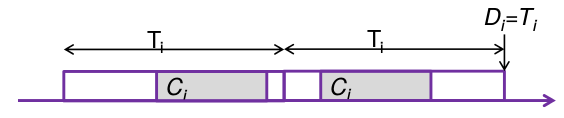
\includegraphics[width=0.5\linewidth]{img/RM.png}
\end{center}

RM is easy to implement with low overhead since task priorities are set at 
design time and does not change during run time but RM does not 
allow high CPU utilization because scheduling too rigid

\paragraph{Worst Case Execution Time}
To know worst case execution we can either do measurement or use static analysis

\subsubsection{Deadline Monotonic Scheduling}

RM does is not good for $D_i < T_i$, so in DM, task with shortest deadline
has highest priority. DM is on \textcolor{red}{optimal} preemptive static priority scheduling
algorithm for $D_i<T_i$.
$$\sum_{i=1}^N \frac{C_i}{D_i}\leq N(2^{\frac{1}{N}}-1)$$

\begin{center}
    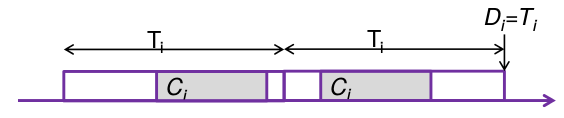
\includegraphics[width=0.5\linewidth]{img/RM.png}
\end{center}

\subsubsection{Response Time Analysis}
RTA provides a sufficient and necessary test for all fixed-priority preemptive 
scheduling algorithms (RM,DM,\ldots)\\
A task set is schedulable if worst-case response time $R_i \leq D_i$ for all tasks.
\begin{itemize}
    \item Response time $R_i$ = $C_i + I_i$ where $I_i$ is the worst
        case interference time = amount of time a task is delayed by
        execution of higher priority tasks
\end{itemize}

\begin{eqnarray}
    R_i =& C_i + I_i\\
    R_i =& C_i + \sum_{j\in hp(i)} \lceil \frac{R_i}{T_j}\rceil C_j
    \label{rta-eq}
\end{eqnarray}

where hp(i) is the set of tasks with higher priotity than task i 
$\to \lceil \frac{R_i}{T_j}\rceil$ is the number of preemptions of task i by task j.



~\eqref{rta-eq} is a recursive formula so it is solve by finding smallest fixed point:
$$R_i^0 = C_i$$
$$R_i^{m+1} = C_i + \sum_{j \in hp(i)} \lceil \frac{R_i^m}{T_j}\rceil C_j$$

\subsubsection{Earliest Deadline First}

Optimal preemptive \textbf{dynamic} priority scheduling algorithm 
where task with earliest absolute deadline has the highest priority. The
absolute deadline is the time when the job is ready + $D_i$.

\subsection{Scheduling with resource lock}

We have assumed that task are independent, in a real systems, tasks can
be dependent because they access a shared resource in a critical section
(CS). In this case, a task with highest priority can be
\textbf{unboundedly} blocked by tasks with lower priority. Response time
becomes: $$R_i = C_i + I_i + B_i$$ where $B_i$ is the time the task is
blocked because a resource has been locked.

\begin{center}
    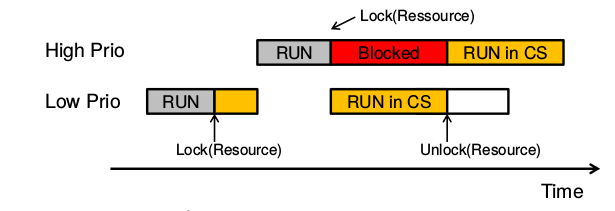
\includegraphics[width=0.5\linewidth]{img/priority.png}
\end{center}

\paragraph{Note:} RTA a test only sufficient, not necessary with blocking.

\paragraph{Priority inversion problem}

\begin{center}
    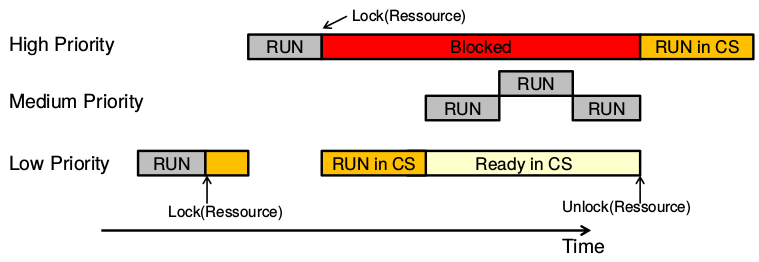
\includegraphics[width=0.5\linewidth]{img/inversion.png}
\end{center}

\subsubsection{Priority Inheritance Protocol}

To avoid this problem, a low-priority task inherits the priority of the 
blocked high-priority task.
\begin{itemize}
    \item When task i is blocked by a CS held by task k 
        and prio(i) > prio(k) $\to$ prio(k) := prio(i)
    \item When task k leaves the CS:
        \begin{itemize}
            \item If task k no longer blocks any tasks, it returns to its old priority
            \item If task k still blocks other tasks, it inherits their highest priority
        \end{itemize}
\end{itemize}

\subsubsection{Priority Ceiling Protocol}
Alternative to priority inheritance, a shared resource R can be accessed
only tasks $S_R = \{ t_1,\ldots,t_m\}$.
\begin{itemize}
    \item Assign a priority ceiling $C_R$ to that resource
        $$C_R = max_{t_i\in S}(prio(t_i))$$
    \item When a task locks that resource, its priority is immediately
        boosted to $C_R$
\end{itemize}

\paragraph{Note:}
Priority inheritance and priority ceiling require a scheduler that can handle
dynamic priorities

\subsection{Aperiodic/sporadic tasks}

\begin{itemize}
    \item \textbf{With hard deadlines}
        \begin{enumerate}
            \item \begin{itemize}
                    \item Take the lowest inter-arrival time L of those tasks
                    \item Treat them as a virtual periodic task with period L in 
                        schedulability analysis
                    \item[$\Rightarrow$]Too pessimistic
                \end{itemize}
        \end{enumerate} 

    \item \textbf{Without hard deadlines}
        \begin{enumerate}
            \item \begin{itemize}
                    \item Maintain the hard deadlines for the periodic tasks
                    \item Try to reduce response time for the other tasks
                \end{itemize}

                Simple and no impact on periodic tasks but possibly very
                long response times if the system is very busy with
                periodic task

            \item Polling server
                \begin{itemize}
                    \item A periodic task (''server'') with period $T_S$ to serve 
                        aperiodic/sporadic requests
                    \item Incoming aperiodic/sporadic jobs are queued in a queue
                    \item In one execution period, the server only runs up to $C_S$ time units
                \end{itemize}
                Performance can be controlled by the period and the priority of the server
                tasks and by $C_S$. 

                \begin{itemize}
                    \item Advantage: Polling server can be treated like a periodic task with
                        WCET $C_S$
                    \item Disadvantage: If an aperiodic/sporadic job is not handled by the
                        server in a time period, it has to wait for the next period $\to$ 
                        response time increases
                    \item Can be extended to multiple servers with different priorities,
                        periods and $C_S$ for different classes/types jobs.
                \end{itemize}
        \end{enumerate}
\end{itemize}


